\documentclass[12pt,a4paper]{article}
\usepackage[latin2]{inputenc}
\usepackage{graphicx}
\usepackage{ulem}
\usepackage{amsmath}
\usepackage[margin=0.5in]{geometry}
\usepackage[T1]{fontenc}
\usepackage[ampersand]{easylist}
\usepackage[english]{babel}
\usepackage{scrextend}
\usepackage{subfig}
\usepackage{float}
\usepackage{stackengine}
\usepackage{listings}
\usepackage{epstopdf}
%\usepackage[demo]{graphicx}
%\usepackage{caption}
%\usepackage{subcaption}
%\usepackage[utf8]{inputenc}
\begin{document}

%%%%%%%%%%%%%%%%%%%%%%%%%%%%%%%%%%%%%%%%%%%%%%%%%%%%%%%%%%%%%%%%%%%%%%%%%%%%%%%%
% Document Setup

\pagenumbering{arabic}

%%%%%%%%%%%%%%%%%%%%%%%%%%%%%%%%%%%%%%%%%%%%%%%%%%%%%%%%%%%%%%%%%%%%%%%%%%%%%%%%
% Title block - Page 0

% Cover page. Clearly indicate the names of the team members.

\author{
  Singireddy, Sanjana\\
  \texttt{sanjana9@stanford.edu}\\
  \texttt{SUID:06030068}
  \and
  Lenius, Samuel\\
  \texttt{lenius@stanford.com}\\
  \texttt{SUID:06091240}
}

\title{2016 EE214B Design Project - Part I}

\maketitle

\pagebreak

%%%%%%%%%%%%%%%%%%%%%%%%%%%%%%%%%%%%%%%%%%%%%%%%%%%%%%%%%%%%%%%%%%%%%%%%%%%%%%%%
% Bias Calculations - Page 2

% Bias point calculations for part I (a). Include a comparison with SPICE
% results from part (b) by providing a table that states the percentage
% deviations in the calculated voltages, g m and rpi.

\section{Bias Calculations}


\subsection{Node Definitions}
\begin{flushleft}

$V_{C1} = V_{E2} = V_{W}$

$V_{B3} = V_{C2} = V_{B4} = V_{X}$

$V_{E3} = V_{Y}$

$V_{E4} = V_{Z}$

$V_{B1} = V_{IN}$

\end{flushleft}

\subsection{Node Voltages and Device Currents}

\begin{equation}
  V_{IN} = V_{BE} = 0.8V
\end{equation}

\begin{equation}
  V_{B2} = 1.6V => V_{W} = 1.6 - V_{BE} = 0.8V
\end{equation}

Assuming Ib = 0
\begin{equation}
  V_{IN} = V_{Y} => V_{Y} = 0.8V
\end{equation}

\begin{equation}
  V_{X} = V_{Y} + V_{BE} => V_{X} = 1.6V
\end{equation}

\begin{equation}
  V_{Z} = V_{X} - V_{BE} => V_{Z} = 0.8V
\end{equation}

\begin{equation}
  V_{O} = V_{CC} - I_{B4} R_{C4} => V_{O} = 2.3V
\end{equation}

\begin{equation}
  I_{C1} = I_{C2} = \frac{V_{CC} - V_{B3}}{R_{C2}} = 3.6mA
\end{equation}

\begin{equation}
  I_{C3} = I_{Bias3} = 4.5mA
\end{equation}

\begin{equation}
  I_{C4} = I_{Bias4} = 2.0mA
\end{equation}

\begin{table}[h]
\centering
\begin{tabular}{|l|l|l|l|}
\hline
Parameter & Hand Calc &  Spice Value & Percent Error\% \\
\hline
$V_{IN}$ & 0.800V &  0.801V &  -0.12\%\\
\hline
$V_{W}$ & 0.800V &  0.798V &  0.25\%\\
\hline
$V_{X}$ & 1.600V &  1.605V &  -0.31\%\\
\hline
$V_{Y}$ & 0.800V &  0.804V &  -0.49\%\\
\hline
$V_{Z}$ & 0.800V &  0.813V &  -1.50\%\\
\hline
$V_{O}$ & 2.300V &  2.301V &  -0.04\%\\
\hline
$gm_{1}$ & 120.7mS & 120.7mS &  -0.03\%\\
\hline
$gm_{2}$ & 120.3mS & 120.3mS &  -0.03\%\\
\hline
$gm_{3}$ & 152.3mS & 152.3mS &  0.02\%\\
\hline
$gm_{4}$ & 70mS & 70mS &  -0.04\%\\
\hline
$r\pi_{1}$ & 2.14k$\Omega$ & 1.875k$\Omega$ &  14.3\%\\
\hline
$r\pi_{2}$ & 2.14k$\Omega$ & 1.883k$\Omega$ &  13.64\%\\
\hline
$r\pi_{3}$ & 1.71k$\Omega$ & 1.502k$\Omega$ &  13.84\%\\
\hline
$r\pi_{4}$ & 3.85k$\Omega$ & 3.515k$\Omega$ &  9.5\%\\
\hline
\end{tabular}
\end{table}

\pagebreak

%%%%%%%%%%%%%%%%%%%%%%%%%%%%%%%%%%%%%%%%%%%%%%%%%%%%%%%%%%%%%%%%%%%%%%%%%%%%%%%%
% Calculations c-f, pages 3-6

\section{Calculations and plots for part I (c) through (f)}

(c) Applying two-port analysis for loop gain calculation gives:

\begin{equation}
  a = (r_{\pi1} || R_{F}) \cdot (-gm_1 R_{C2} ) \cdot \frac{gm_3 R_F}{1 + gm_3 R_F} = -5.486k\Omega
\end{equation}

\begin{equation}
  f = \frac{-1}{R_F} = -4.5mS
\end{equation}

\begin{equation}
  T_{0} = a f = 26.57 = 28.48dB
\end{equation}

Mid-band transresistance of the overall amplifier:

\begin{equation}
  A_{CL, MidBiand} = \frac{a}{1 + T_0} \cdot \frac{-gm_4 R_{C4}}{1 + gm_4 R_{E4}} = 724 = 57.2dB
\end{equation}

\newpage
(d) Calculating node resistances and capacitances to estimate the poles at the nodes:

At node X, $C_{\pi 3}, C_{\pi 4}, r_{\pi 3}$ and $r_{\pi 4}$ will be bootstrapped due to the presence of emitter degeneration resistances.

Miller approximation was applied to $C_{\mu 4}$

\begin{equation}
  C_X = C_{\mu 2} + \frac{C_{\pi 3}}{1 + gm_3 R_F} + \frac{C_{\pi 4}}{1+gm_4 R_{E4}} + C_{\mu 3} + C_{\mu 4} (1 + gm_4 R_{C4}) = 99fF
\end{equation}

\begin{equation}
  R_X = R_{C2} || r_{\pi 3}(1+gm_3 R_F) || r_{\pi4}(1+gm_4 R_{E4}) = 241\Omega \approx R_{C2}
\end{equation}

\begin{equation}
  C_{IN} = C_D + C_{\pi1} + C_{\mu1} = 324fF
\end{equation}

\begin{equation}
  R_{IN} = r_{\pi1} || R_F = 199\Omega \approx R_F
\end{equation}

The two most significant poles are given by:

\begin{equation}
  f_{IN} = \frac{1}{2 \pi R_{IN} C_{IN}} = 2.46GHz
\end{equation}

\begin{equation}
  f_{X} = \frac{1}{2 \pi R_{X} C_{X}} = 6.63GHz
\end{equation}

\newpage
(e) Calculation of $T(j\omega)$ Unity Gain Frequency and Phase Margin

\begin{equation}
  f_{u} = \sqrt{T_0 * f_{IN} * f_{X}} = 20.8GHz
\end{equation}

\begin{equation}
  PM = 180\textdegree  - atan(\frac{f_u}{f_{IN}}) - atan(\frac{f_u}{f_{X}}) = 24.4\textdegree
\end{equation}

{\centering
	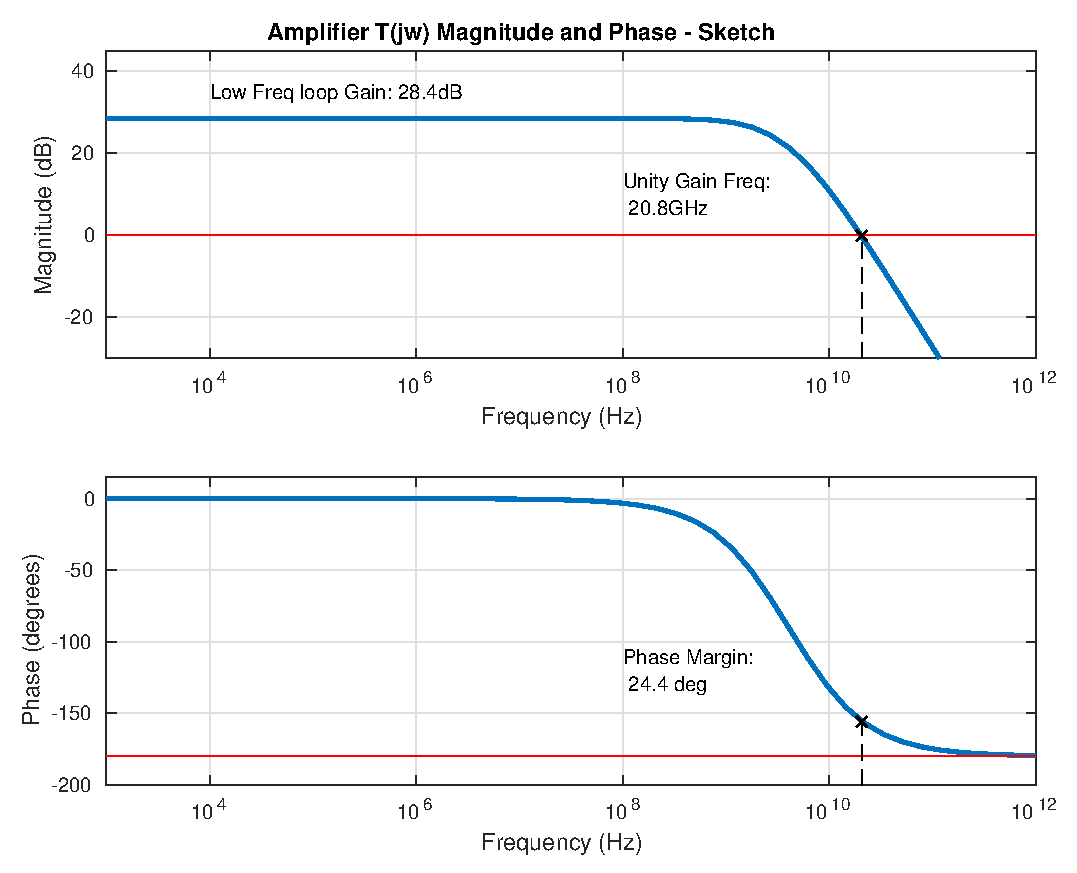
\includegraphics[width=0.8\textwidth]{plots/part_e.eps}
\par}

The low value of phase margin suggests that significant peaking will be observed.

\newpage
(f) Assuming a two pole loop response, the closed loop transimpedance and pole locations are given by:

\begin{equation}
  a(s) = (R_{IN} || \frac{1}{sC_{IN}}) \cdot gm_1 \cdot (R_X || \frac{1}{sC_X}) \cdot \frac{gm_3 R_f}{1 + gm_3 R_F}
\end{equation}

\begin{equation}
  T(s) = \frac{T_{0}}{(1 + \frac{s}{\omega_X})(1+\frac{s}{\omega_{IN}})}
\end{equation}

\begin{equation}
  A(s) = \frac{v_{E3}}{i_s} = \frac{a(s)}{1 + a(s) f} = \frac{1}{f} \cdot \frac{T(s)}{1 + T(s)}
\end{equation}
Simplifying the above equation gives

\begin{equation}
  A(s) = \frac{A_0}{1 + \frac{s}{\omega_0 Q} + \frac{s^{2}}{\omega_0^{2}}} 
\end{equation}
 
where,

\begin{equation}
  \omega_{0} = \sqrt{(1+T_0) * \omega_{IN} * \omega_{X}} 
\end{equation}

\begin{equation}
  Q = \frac{\sqrt{(1 + T_0) \omega_{X} \omega_{IN}}}{\omega_X + \omega_{IN}}
\end{equation}

Substituting the values of $T_0$ and $\omega_X$ and $\omega_{IN}$ from parts (c) and (d) gave 

\begin{equation}
  \omega_{0} = 133.32 G rad s^{-1}
% To Do: Add value of w_0
\end{equation}

\begin{equation}
  Q = 2.29
\end{equation}

Once $Q$ and $\omega_0$ are obtained, the poles are obtained by solving the equation:

\begin{equation}
  \frac{s^{2}}{\omega_0^{2}} + \frac{s}{\omega_0 Q} + 1 = 0
\end{equation}

The real and imaginary pole locations obtained are 
\begin{equation}
  Re(\frac{s}{2 \pi}) = -4.705 GHz
\end{equation}

\begin{equation}
  Im(\frac{s}{2 \pi}) = 20.69 GHz
\end{equation}
Hence the pole locations are (-4.705 $\pm$ 20.69) GHz


\pagebreak


%%%%%%%%%%%%%%%%%%%%%%%%%%%%%%%%%%%%%%%%%%%%%%%%%%%%%%%%%%%%%%%%%%%%%%%%%%%%%%%%
% Bode Diagrams - Page 7 & 8

% Bode plot and pz outputs for parts I (g) and (h). Be sure to include proper
% annotations, and comparisons to hand calculated values.

\section{Bode Plots and PZ Outputs - Part I(g,h)}

{\centering
	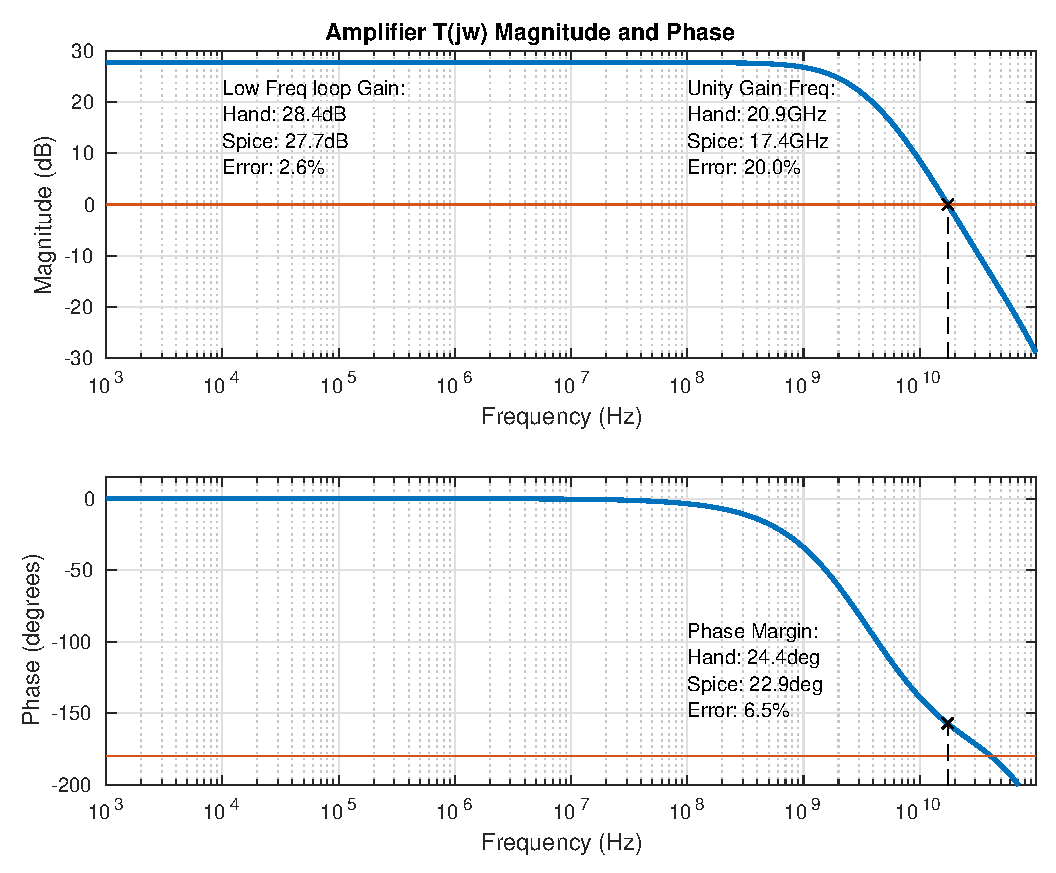
\includegraphics[width=0.8\textwidth]{plots/part_g.eps}
\par}

\pagebreak

{\centering
	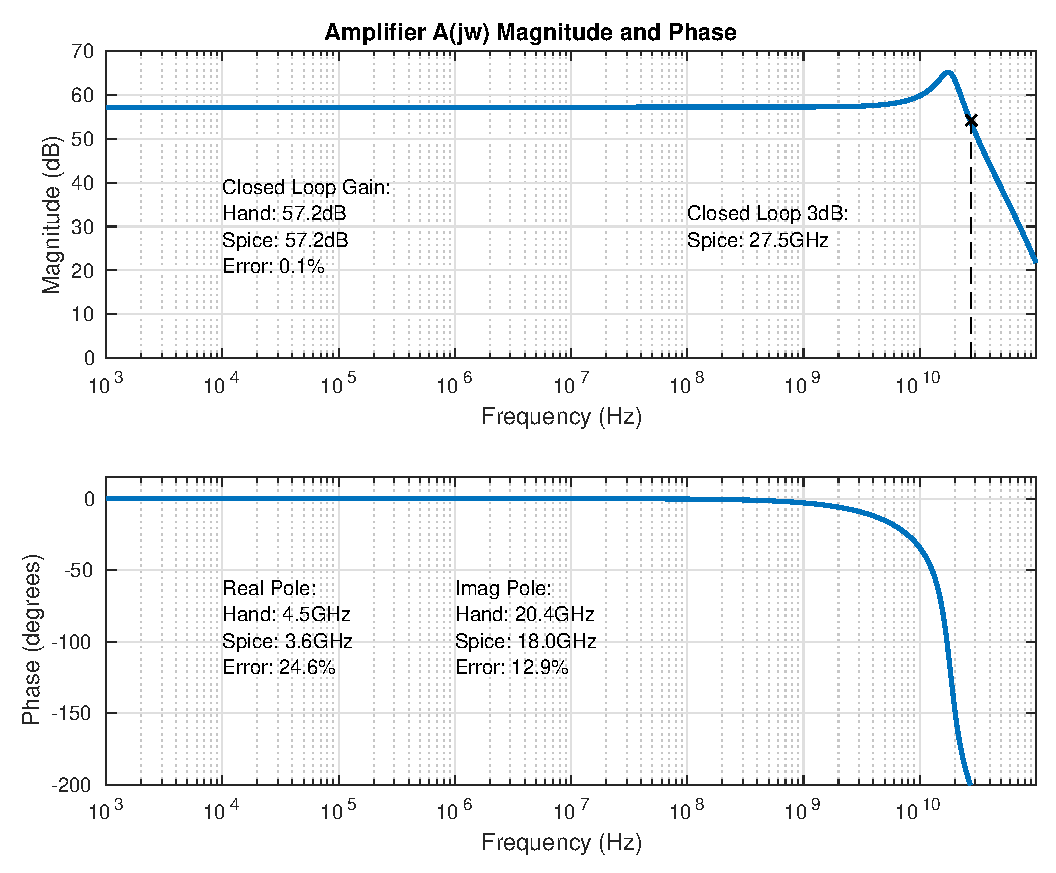
\includegraphics[width=0.8\textwidth]{plots/part_h.eps}
\par}

\begin{verbatim}
 ***************************************************
    ******   pole/zero analysis
    input =  0:is          output = v(vo)
    poles (rad/sec)                 poles ( hertz)
    real            imag            real            imag
    -33.1562m       0.              -5.27698m       0.
    -22.9305g       113.319g        -3.64950g       18.0353g
    -22.9305g       -113.319g       -3.64950g       -18.0353g
    -473.782g       0.              -75.4048g       0.
    -1.12800t       0.              -179.526g       0.
    -1.18039t       0.              -187.865g       0.

    zeros (rad/sec)                 zeros ( hertz)
    real            imag            real            imag
    0.              0.              0.              0.
    -1.10418t       0.              -175.736g       0.

\end{verbatim}

\pagebreak

%%%%%%%%%%%%%%%%%%%%%%%%%%%%%%%%%%%%%%%%%%%%%%%%%%%%%%%%%%%%%%%%%%%%%%%%%%%%%%%%
% Calculations for part I (i). - Page 9

\section{Calculations for Part I(i)}

% part i
% The capacitor Cf can be used to introduce a feedback zero. Estimate the value
% of Cf that yields a maximally flat response. What is the expected closed-loop
% bandwidth of the circuit?

%f_o = 1.7443184E+10;
%w_o = f_o * 2 * pi;
%w_z = w_o / sqrt(2);
%w_z = w_o / (sqrt(2) - (pole.vi.w + pole.vx.w) / w_o);
%c_z = 1 / (w_z * r_f);

%c_in_z = c_in + c_z;
%cl_3db_w = sqrt((1+k) / (r_in * c_in_z * r_x * c_x));
%cl_3db_f = cl_3db_w / (2 * pi);
A feedback capacitor can be used to introduce a zero into the feedback loop in
order to push the higher frequency pole out and flatten the response of the
closed loop amplifier. The optimally flat response of the amplifier occurs when Q = $\sqrt{2}$. Hence:

\begin{equation}
  \omega_0 = 1.09e11 rad/s
\end{equation}

\begin{equation}
  \omega_Z = \frac{\omega_{0}}{\sqrt{2} - \frac{\omega_{P1} + \omega_{P2}}{\omega_{0}}}
\end{equation}

\begin{equation}
  C_F = \frac{1}{\omega_Z R_F} = 37fF
\end{equation}

From this, the new closed loop bandwidth can be calculated as such:

\begin{equation}
  C_{in,C_F} = C_{in} + C_F
\end{equation}

\begin{equation}
  k = \frac{R_{in} * Q1_{gm} * R_x * A_{V3}}{R_F}
\end{equation}

\begin{equation}
  BW_{CL,C_F} = \frac{\sqrt{1 + k}}{2 \pi R_{in} C_{in} R_x C_x} = 19.2Ghz
\end{equation}

Value of $C_F$ was tweaked from 37fF to 45fF in order to flatten the magnitude response. Approximately 0.1dB of peaking was observed in the response curve, and with 45fF it was completely flat. We noted that on the output noise plot there was a significant bump in noise around the 3dB frequency that could be reduced by increasing $C_F$ however this was not a specified goal of the design, so we chose to leave the value as-is.
\pagebreak


%%%%%%%%%%%%%%%%%%%%%%%%%%%%%%%%%%%%%%%%%%%%%%%%%%%%%%%%%%%%%%%%%%%%%%%%%%%%%%%%
% Bode Diagrams - Page 10 & 11

% Bode plots and pz outputs for part I (j). Be sure to include proper
% annotations, and comparisons to hand calculated values.

\section{Bode Plots and PZ Outputs - Part I(j)}

%{\centering
	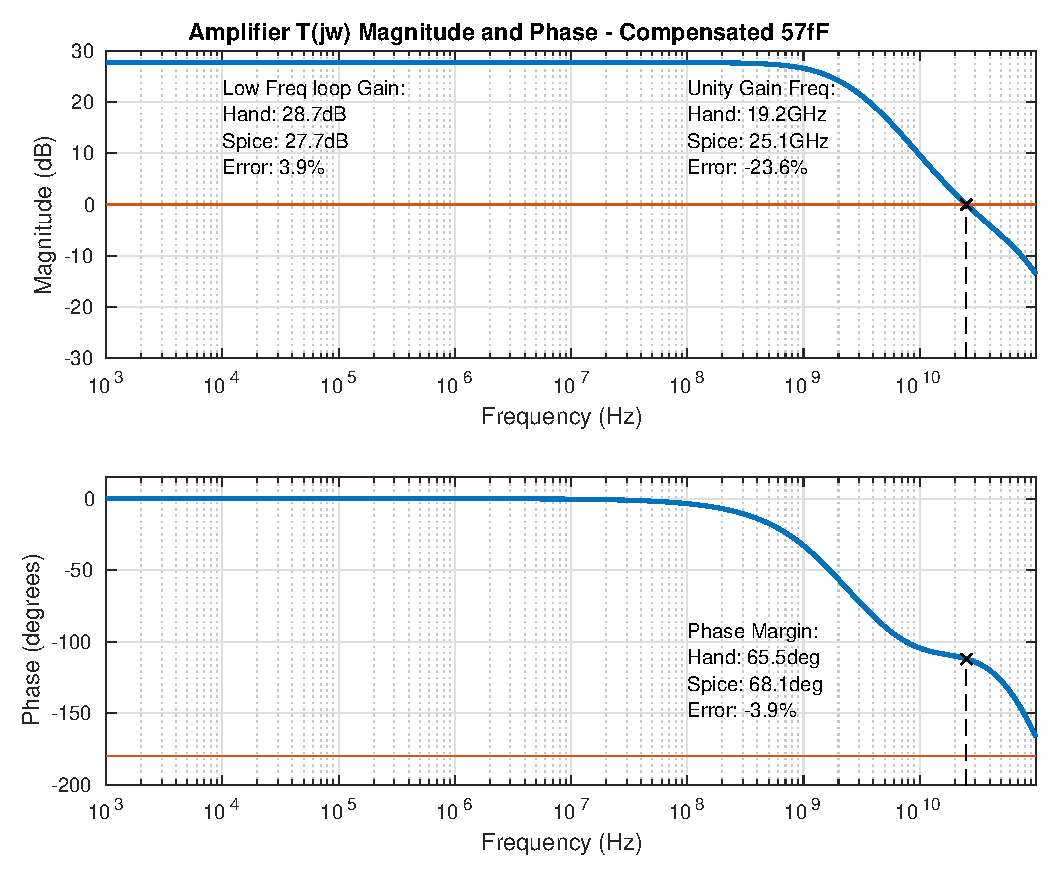
\includegraphics[width=0.8\textwidth]{plots/part_j_t.eps}
%\par}

\pagebreak

{\centering
	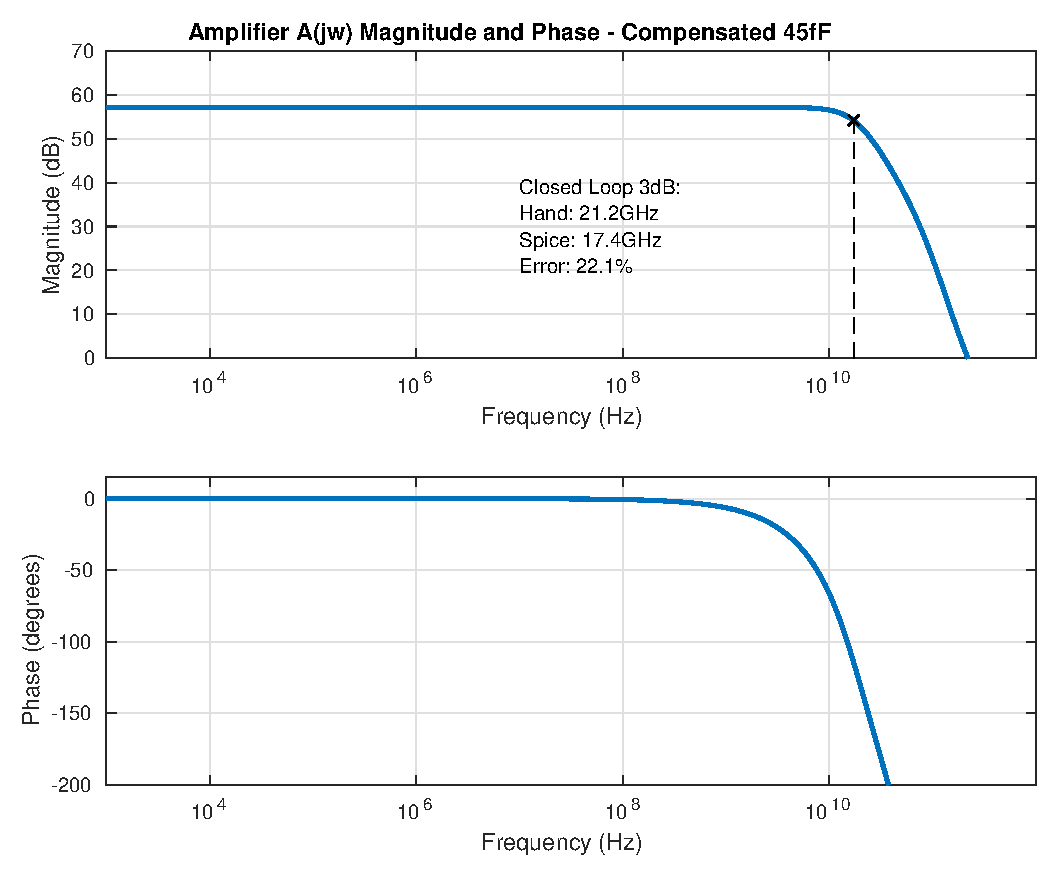
\includegraphics[width=0.8\textwidth]{plots/part_j_a.eps}
\par}

\begin{verbatim}
 ***************************************************
    ******   pole/zero analysis


    input =  0:is          output = v(vo)

    poles (rad/sec)                 poles ( hertz)
 real            imag            real            imag            
 -33.1562m       0.              -5.27698m       0.              
 -86.5643g       75.6614g        -13.7771g       12.0419g        
 -86.5643g       -75.6614g       -13.7771g       -12.0419g       
 -385.396g       343.565g        -61.3377g       54.6800g        
 -385.396g       -343.565g       -61.3377g       -54.6800g       
 -1.11884t       0.              -178.069g       0.              
 -1.35144t       0.              -215.088g       0.              
 -1.90665t       0.              -303.452g       0.              

 zeros (rad/sec)                 zeros ( hertz)
 real            imag            real            imag            
 0.              0.              0.              0.              
 -1.09715t       0.              -174.617g       0.

\end{verbatim}

\pagebreak

%%%%%%%%%%%%%%%%%%%%%%%%%%%%%%%%%%%%%%%%%%%%%%%%%%%%%%%%%%%%%%%%%%%%%%%%%%%%%%%%
% Noise - Page 12

% Calculations and simulation plot (with proper annotation) for parts I (k)
% and (l).

\section{Noise - Part I(k,l)}

{\centering
	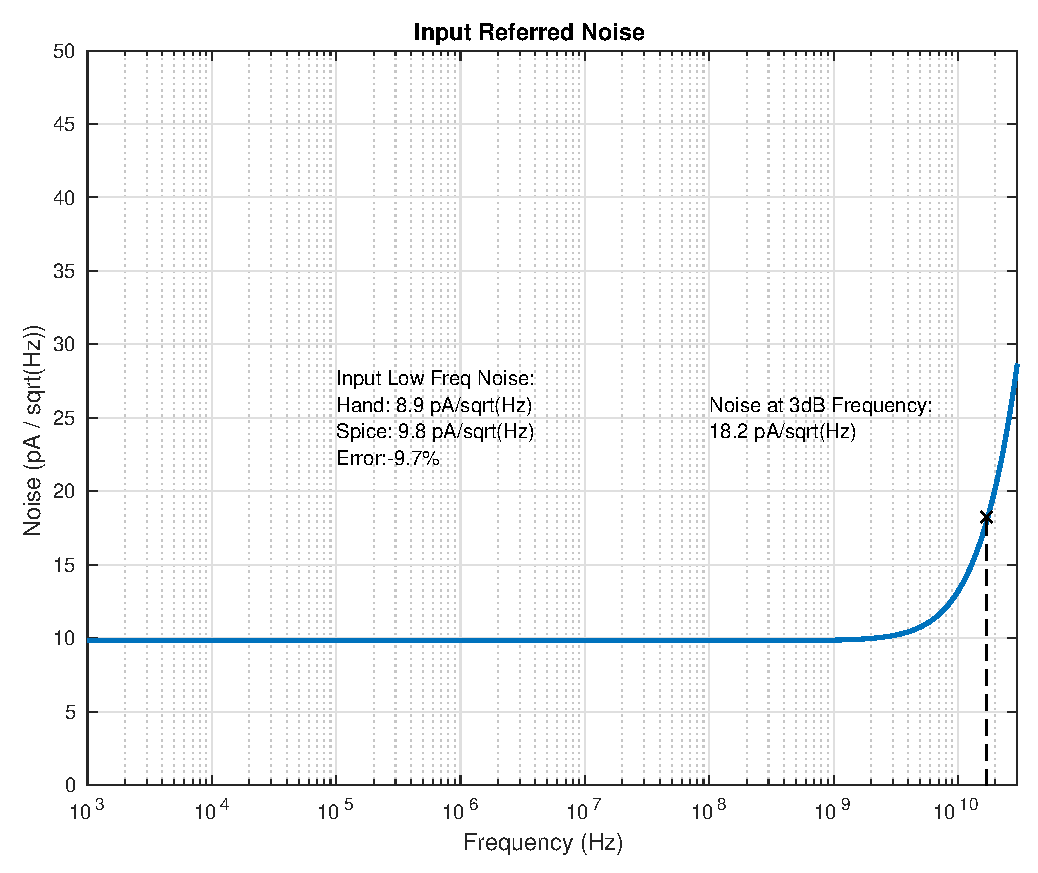
\includegraphics[width=0.8\textwidth]{plots/part_l.eps}
\par}

\pagebreak

%%%%%%%%%%%%%%%%%%%%%%%%%%%%%%%%%%%%%%%%%%%%%%%%%%%%%%%%%%%%%%%%%%%%%%%%%%%%%%%%
% Transient Rresponse - Page 13

\section{Transient Response - Part I(m)}

{\centering
	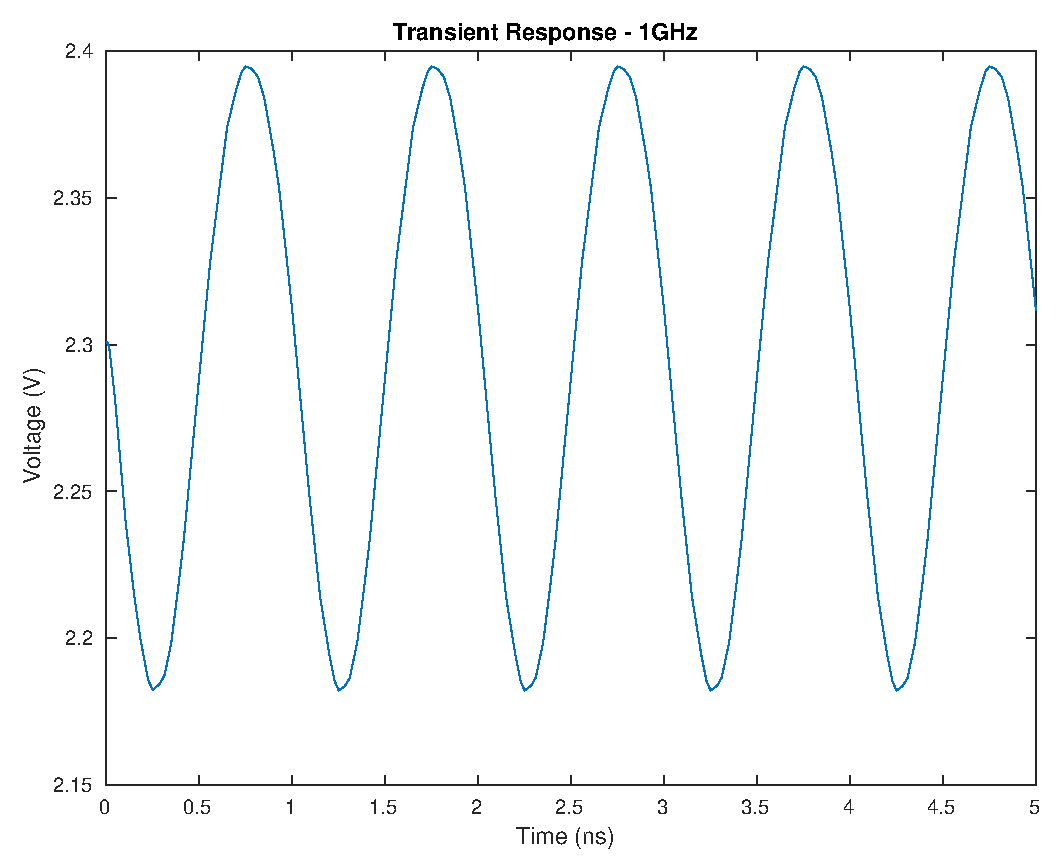
\includegraphics[width=0.8\textwidth]{plots/part_m.eps}
\par}

\pagebreak

\end{document}
